\section{Discussion and Conclusion}
\label{sec:conclusion}
%
\paragraph{Limitations and future work}
While taking into account the effect of the near-field on clusters, our work is still based on the RTT. Therefore it relies on the far-field approximation to represent a scattering dyad useful for rendering. Therefore, while we can handle near- and far-field scattering, we cannot accurately model the scattering in the intermediate region, which we treat as the far field. Using more accurate representations, that capture the effects at such near-field region could further enhance the generality of our theory and, thus, is an interesting future topic. This would however require exploring an alternative light transport framework beyond the RTT.

Right now, our implementation requires precomputing the bulk optical properties of the media. This limits the applicability of our work to media with homogeneous particle statistical properties. Finding faster approximations for our scattering functions, in the same spirit as the geometric optics approximation for Lorenz-Mie theory~\cite{glantschnig1981light}, is an interesting future research. 

Finally, our implementation is currently limited in practice to spherical particles with identical radii within a particle cluster. Allowing general and spatially varying particle shapes by using an alternative implementation of the T-matrix method would further improve the versatility of our technique.

\paragraph{Conclusion}
In this paper, we introduce a new technique to systematically compute bulk scattering parameters for participating media. Built upon first principles of light transport (i.e., Maxwell electromagnetism), our technique models a translucent material as clusters of particles randomly distributed in embedding media. Our work generalizes the widely-used Lorenz-Mie theory for rigorously deriving optical properties of scattering media, and can be readily used in any radiative-based light transport simulator. 
%
We have demonstrated the significant effects of departing from the underlying assumptions of Lorenz-Mie theory, and the versatility for modeling a wide range of participating media by modifying the arrangement of particles within each cluster, including isotropic, anisotropic, and correlated media.

\begin{figure}
    \centering
    \setlength{\resLen}{0.8in}
    \addtolength{\tabcolsep}{-3.5pt}
    \small
    %
    \begin{tabular}{cc|cc}
        \multicolumn{2}{c|}{(a) \textbf{Negatively correlated} particles} &
        \multicolumn{2}{c}{(b) \textbf{Positively correlated} particles}
        \\
        \multicolumn{2}{c|}{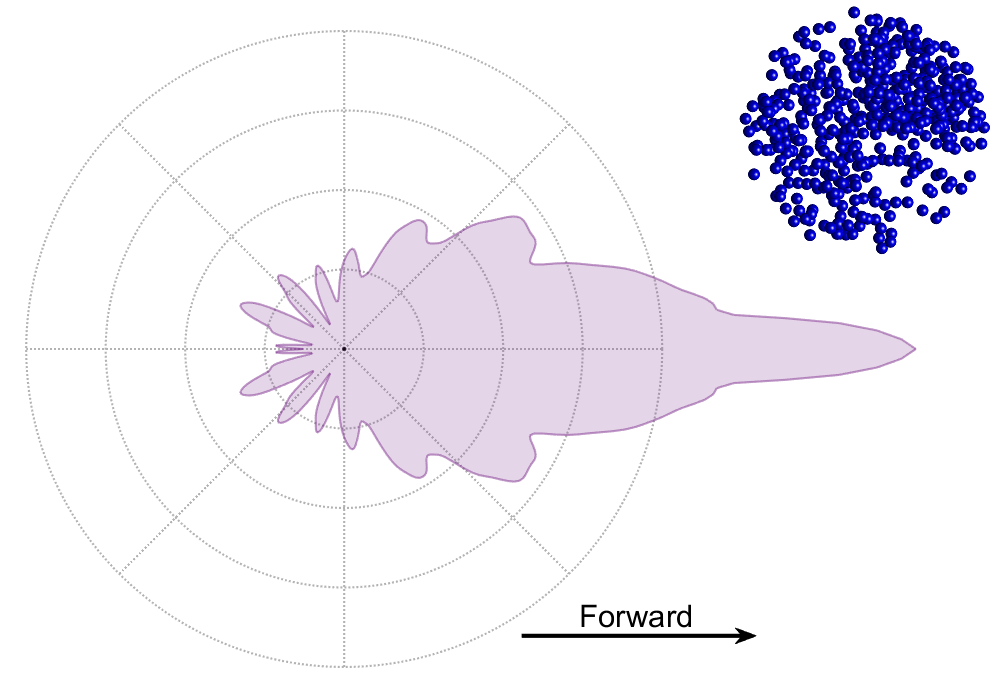
\includegraphics[width=2\resLen]{images/pfunc/negative.png}} & \multicolumn{2}{c}{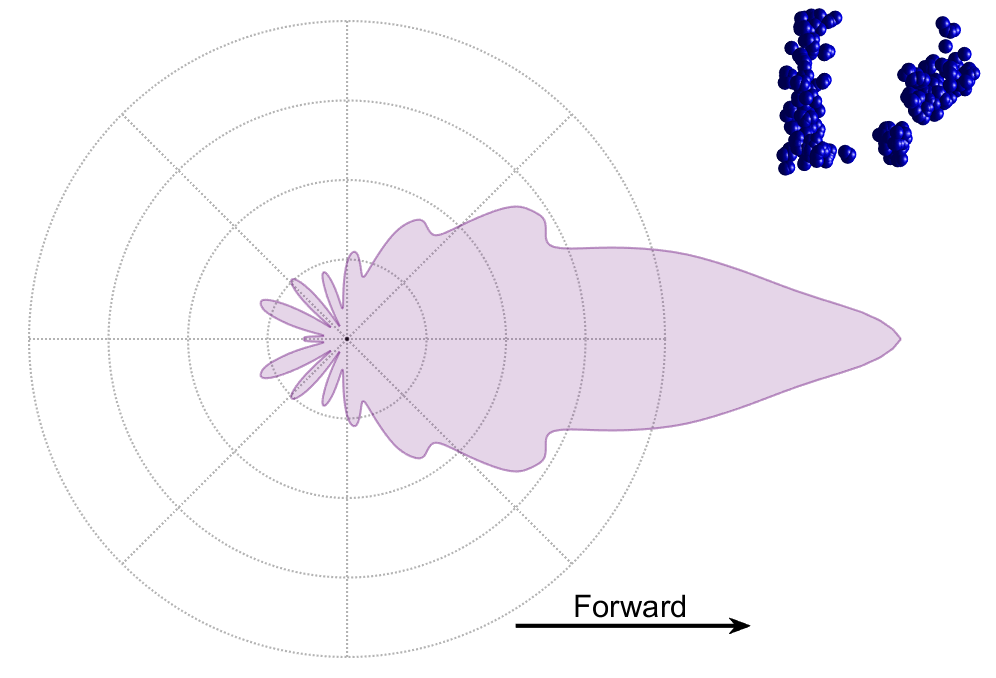
\includegraphics[width=2\resLen]{images/pfunc/positive.png}} 
        \\
        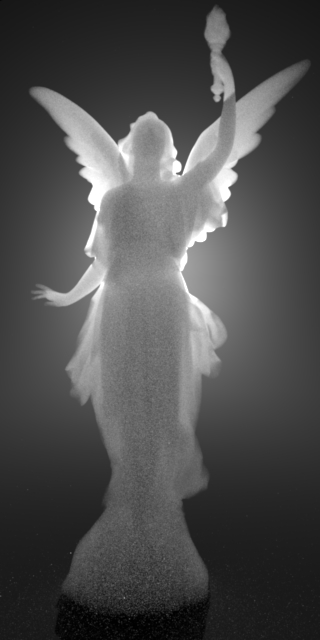
\includegraphics[width=\resLen]{images/lucy/neg_unc.jpg} &
        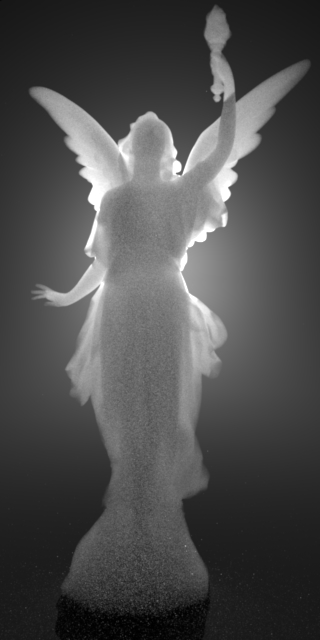
\includegraphics[width=\resLen]{images/lucy/neg_neg.jpg} &
        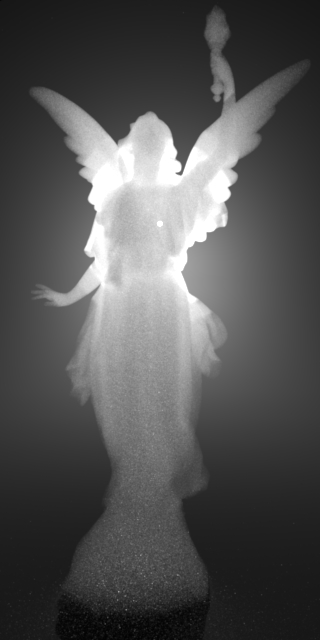
\includegraphics[width=\resLen]{images/lucy/pos_unc.jpg} &
        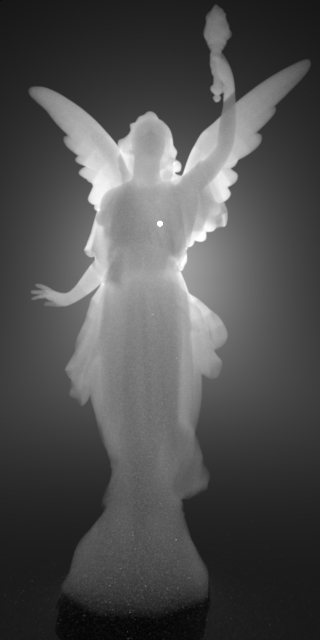
\includegraphics[width=\resLen]{images/lucy/pos_pos.jpg} 
        \\
        (a1) \textbf{unc.} clusters & (a2) \textbf{neg.} clusters & (b1) \textbf{unc.} clusters & (b2) \textbf{pos.} clusters
    \end{tabular}
    \caption{\label{fig:correlated}
        By correlating particle positions negatively (a) or positively (b), our method can produce bulk scattering parameters for near-field correlated media.
        In this example, we use $\lambda = 400\text{nm}$, particle radius~$\radius_i = 500\text{nm}$, and per-cluster particle count $\Ncls = 100$.
        Additionally, we can further correlate particle clusters themselves, a variety of appearances can be achieved (a1--b2).
        (The bright dot in (b1) and (b2) emerges from unscattered light from the area source.)
    }
\end{figure}


